\documentclass{article}
\usepackage{graphicx}
\usepackage{float}
\begin{document}
\begin{titlepage}
\begin{center}
\huge{\bfseries My Report On}\\
\huge{\bfseries Mathematics}\\
\line(1,0){400}\\
\textsc{\LARGE LaTeX report}\\
\end{center}

\begin{flushright}
\textsc{\LARGE A S M Masud Parvez\\}
Department of Computer Science and Engineering\\
ID:18ICTCSE035\\
E-mail:parvezcse35@gmail.com\\
Phone:01864910087\\
\end{flushright}

\end{titlepage}

\tableofcontents
\thispagestyle{empty}
\cleardoublepage


\setcounter{page}{1}
\section{Mathematics}
\begin{figure}[H]
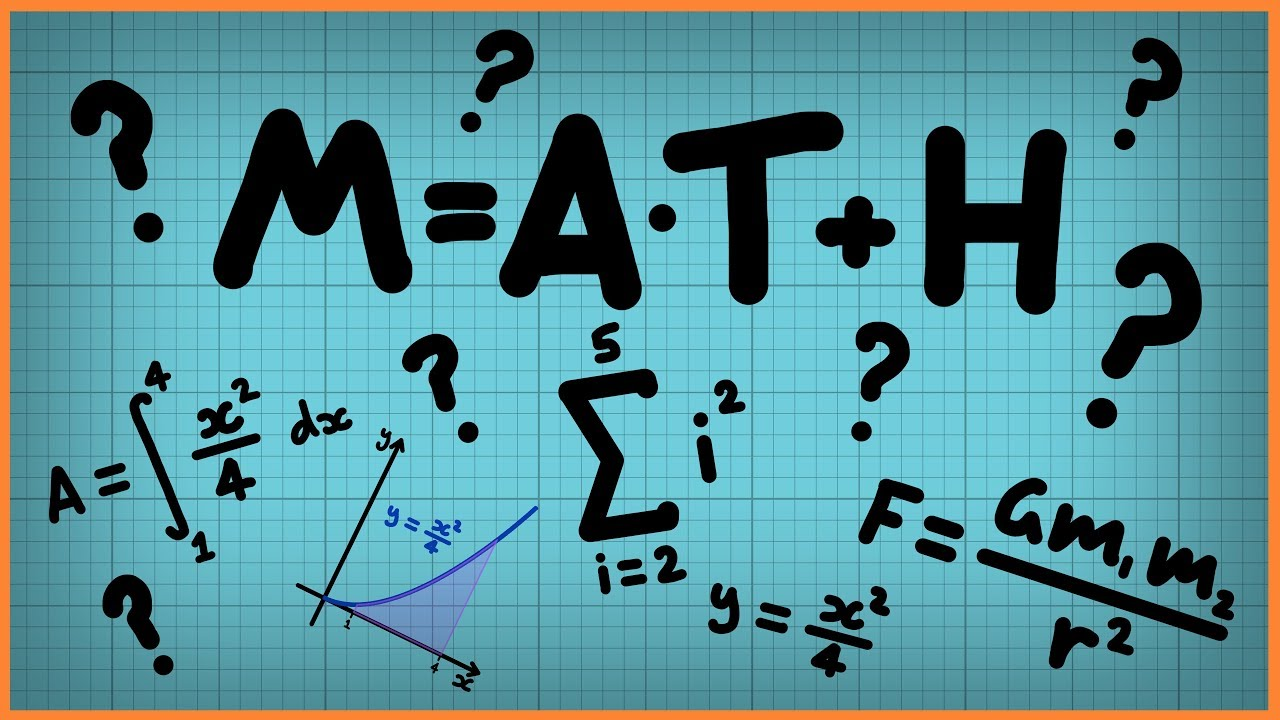
\includegraphics[height=2.5in]{E:/18ICTCSE039 report/math.jpg}
\end{figure}

\section{Introduction}
Mathematics is the science that deals with the logic of shape, quantity and arrangement. Math is all around us, in everything we do. It is the building block for everything in our daily lives, including mobile devices, architecture (ancient and modern), art, money, engineering, and even sports.\newline \newline
Since the beginning of recorded history, mathematic discovery has been at the forefront of every civilized society, and in use in even the most primitive of cultures. The needs of math arose based on the wants of society. The more complex a society, the more complex the mathematical needs. Primitive tribes needed little more than the ability to count, but also relied on math to calculate the position of the sun and the physics of hunting.
\section{History of mathematics}
Several civilizations — in China, India, Egypt, Central America and Mesopotamia — contributed to mathematics as we know it today. The Sumerians were the first people to develop a counting system. Mathematicians developed arithmetic, which includes basic operations, multiplication, fractions and square roots. The Sumerians’ system passed through the Akkadian Empire to the Babylonians around 300 B.C. Six hundred years later, in America, the Mayans developed elaborate calendar systems and were skilled astronomers. About this time, the concept of zero was developed.\newline \newline 
As civilizations developed, mathematicians began to work with geometry, which computes areas and volumes to make angular measurements and has many practical applications. Geometry is used in everything from home construction to fashion and interior design.\newline \newline
Geometry went hand in hand with algebra, invented in the ninth century by a Persian mathematician, Mohammed ibn-Musa al-Khowarizmi. He also developed quick methods for multiplying and diving numbers, which are known as algorithms — a corruption of his name.\newline \newline
Algebra offered civilizations a way to divide inheritances and allocate resources. The study of algebra meant mathematicians were solving linear equations and systems, as well as quadratics, and delving into positive and negative solutions. Mathematicians in ancient times also began to look at number theory. With origins in the construction of shape, number theory looks at figurate numbers, the characterization of numbers, and theorems.
\section{Development of calculus}
In the 17th century, Isaac Newton and Gottfried Leibniz independently developed the foundations for calculus. Calculus development went through three periods: anticipation, development and rigorization. In the anticipation stage, mathematicians were attempting to use techniques that involved infinite processes to find areas under curves or maximize certain qualities. In the development stage, Newton and Leibniz brought these techniques together through the derivative and integral. Though their methods were not always logically sound, mathematicians in the 18th century took on the rigorization stage, and were able to justify them and create the final stage of calculus. Today, we define the derivative and integral in terms of limits.\newline \newline

In contrast to calculus, which is a type of continuous mathematics, other mathematicians have taken a more theoretical approach. Discrete mathematics is the branch of math that deals with objects that can assume only distinct, separated value. Discrete objects can be characterized by integers, whereas continuous objects require real numbers. Discrete mathematics is the mathematical language of computer science, as it includes the study of algorithms. Fields of discrete mathematics include combinatorics, graph theory, and the theory of computation.\newline \newline

People often wonder what relevance mathematicians serve today. In a modern world, math such as applied mathematics is not only relevant, it's crucial. Applied mathematics is the branches of mathematics that are involved in the study of the physical, biological, or sociological world. The idea of applied math is to create a group of methods that solve problems in science. Modern areas of applied math include mathematical physics, mathematical biology, control theory, aerospace engineering, and math finance. Not only does applied math solve problems, but it also discovers new problems or develops new engineering disciplines. Applied mathematicians require expertise in many areas of math and science, physical intuition, common sense, and collaboration. The common approach in applied math is to build a mathematical model of a phenomenon, solve the model, and develop recommendations for performance improvement.\newline \newline

While not necessarily an opposite to applied mathematics, pure mathematics is driven by abstract problems, rather than real world problems. Much of what's pursued by pure mathematicians can have their roots in concrete physical problems, but a deeper understanding of these phenomena brings about problems and technicalities. These abstract problems and technicalities are what pure mathematics attempts to solve, and these attempts have led to major discoveries for mankind, including the Universal Turing Machine, theorized by Alan Turing in 1937. The Universal Turing Machine, which began as an abstract idea, later laid the groundwork for the development of the modern computer. Pure mathematics is abstract and based in theory, and is thus not constrained by the limitations of the physical world.\newline \newline

According to one pure mathematician, pure mathematicians prove theorems, and applied mathematicians construct theories. Pure and applied are not mutually exclusive, but they are rooted in different areas of math and problem solving. Though the complex math involved in pure and applied mathematics is beyond the understanding of most average Americans, the solutions developed from the processes have affected and improved the lives of all.
\newpage
\section{Algebra}
\begin{figure}[H]

\includegraphics[height=2.5in]{E:/18ICTCSE039 report/algebra.jpg}
\end{figure}
\subsection{Overview of Algebra}
Learn the basics of algebra from former USA Mathematical Olympiad winner and Art of Problem Solving founder Richard Rusczyk. Topics covered in the book include linear equations, ratios, quadratic equations, special factorizations, complex numbers, graphing linear and quadratic equations, linear and quadratic inequalities, functions, polynomials, exponents and logarithms, absolute value, sequences and series, and much more!
\newline \newline
The text is structured to inspire the reader to explore and develop new ideas. Each section starts with problems, giving the student a chance to solve them without help before proceeding. The text then includes solutions to these problems, through which algebraic techniques are taught. Important facts and powerful problem solving approaches are highlighted throughout the text. In addition to the instructional material, the book contains well over 1000 problems. The solutions manual contains full solutions to all of the problems, not just answers.
\newline \newline 
This book can serve as a complete Algebra I course, and also includes many concepts covered in Algebra II. Middle school students preparing for MATHCOUNTS, high school students preparing for the AMC, and other students seeking to master the fundamentals of algebra will find this book an instrumental part of their mathematics libraries.
\subsection{Some Equation of Algebra}
1.$$2x^2+3xy+y^2=0$$
2.$$5x^2+13x+45=0$$

\section{Trigonometry}
\begin{figure}[H]
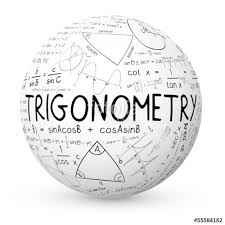
\includegraphics[height=2.5in]{E:/18ICTCSE039 report/trigonometry.jpg}
\end{figure}

\subsection{Overview of Trigonometry}
Trigonometry (from Greek trigōnon "triangle" + metron "measure") is a branch of mathematics that studies triangles and the relationships between the lengths of their sides and the angles between those sides.
\newline \newline
In simple words, we can say that,"Trigonometry is the study of triangle."
\subsection{What is triangle?}
A triangle is a basic geometric shape having three vertices, three sides (edges) and three angles.
\newline \newline
A triangle with three vertices A,B and C as shown in this figure is commonly denoted as ΔABC. a, b, c are three sides of the triangle whereas A, B and C denote the three angles. One simple identity holds for the angles of all types of triangles:
\begin{figure}[H]
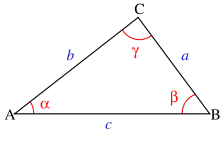
\includegraphics[height=2.5in]{E:/18ICTCSE039 report/triangle.png}
\end{figure}
$$A+B+C=180(degree)$$\\
\subsection{Different Types of Triangles?}
\begin{figure}[H]

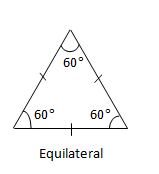
\includegraphics[height=1.5in]{E:/18ICTCSE039 report/equilateral.png}
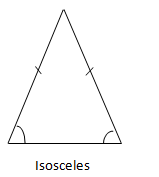
\includegraphics[height=1.5in]{E:/18ICTCSE039 report/isosceles.png}
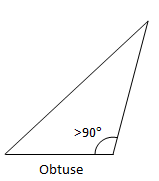
\includegraphics[height=1.5in]{E:/18ICTCSE039 report/obtuse.png}
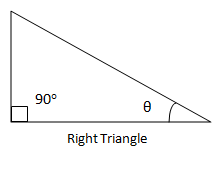
\includegraphics[height=1.5in]{E:/18ICTCSE039 report/rignt-triangle.png}
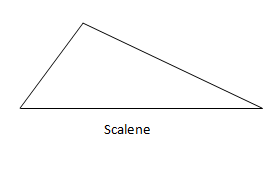
\includegraphics[height=1.5in]{E:/18ICTCSE039 report/scalene.png}
\end{figure}

\newpage
\subsection{Right Angle Triangle}
This special type of triangle has one of the three angles equal to 90∘ and this angle is demonstrated by a small square inside the triangle. C can be any angle..
\begin{figure}[H]
\includegraphics[height=2.5in]{G:/somokoni-tribhuj.jpg}
\end{figure}
Note that the side of the triangle adjacent to angle C is named as adjacent (A). The side opposite to angle C is named as Opposite(O), whereas the third (longest) side is named as Hypotenuse(H).

\subsection{Trigonometric Ratios}
$$SinC=\frac{b}{c}$$\\
$$CosC=\frac{a}{c}$$\\
$$tanC=\frac{b}{a}$$\\
$$SecC=\frac{c}{a}$$\\
$$CosecC=\frac{c}{b}$$\\
$$CotC=\frac{a}{b}$$\\
\begin{table}
\centering
\caption[optional caption]{real, local caption}
\label{tab:tab1}
\begin{tabular}{l c r}
Ratio&Angle\\ \hline
\end{tabular}
\end{table}
\newpage
\section{Geometry}
Geometry is another important topic in mathematics.\\ In modern times, geometry concept have been generalized to a high level of abstraction and complexity and have been subjected to the method of calculus and abstract algebra, so that many modern branches of the field are barely recognizable as the descendants of early geometry.
\subsection{Overview of Geometry}
Learn the fundamentals of geometry from former USA Mathematical Olympiad winner Richard Rusczyk. Topics covered in the book include similar triangles, congruent triangles, quadrilaterals, polygons, circles, funky areas, power of a point, three-dimensional geometry, transformations, and much more.
\newline \newline
The text is structured to inspire the reader to explore and develop new ideas. Each section starts with problems, so the student has a chance to solve them without help before proceeding. The text then includes solutions to these problems, through which geometric techniques are taught. Important facts and powerful problem solving approaches are highlighted throughout the text. In addition to the instructional material, the book contains over 900 problems. The solutions manual contains full solutions to all of the problems, not just answers.
\newline \newline
This book can serve as a complete geometry course, and is ideal for students who have mastered basic algebra, such as solving linear equations. Middle school students preparing for MATHCOUNTS, high school students preparing for the AMC, and other students seeking to master the fundamentals of geometry will find this book an instrumental part of their mathematics libraries.
\subsection{Some Important Equation of Geometry}
Standard equation of Circle:
$$x^2+y^2+2gx+2fy+c=0$$
Equation of Stright line:
$$Y=mX+C$$
\newpage


\section{Calculus}
\begin{figure}[H]
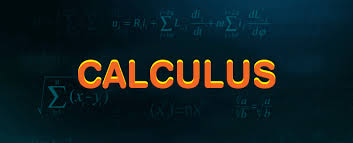
\includegraphics[height=2.5in]{E:/18ICTCSE039 report/calculus.jpg}
\end{figure}
\subsection{Overview of Calculus}
Calculus is part of the acclaimed Art of Problem Solving curriculum designed to challenge high-performing middle and high school students. Calculus covers all topics from a typical high school or first-year college calculus course, including: limits, continuity, differentiation, integration, power series, plane curves, and elementary differential equations. The text is written to challenge students at a much deeper level than a traditional high school or first-year college calculus course.
\newline \newline
The book includes hundreds of problems, ranging from routine exercises to extremely challenging problems drawn from major mathematics competitions such as the Putnam Competition and the Harvard-MIT Math Tournament. Many of the problems have full, detailed solutions in the text, and the rest have full solutions in the accompanying Solutions Manual.
\end{document}